Para el caso de uso de Create task siguiendo\ref{par:testing}

Primero tenemos que localizar los factores o variables independientes

\begin{itemize}
    \item Host
    \item Port
    \item CommunicationMode
    \item ExecutionMode
    \item Steps
\end{itemize}

luego las clases de equivalencia:

\begin{itemize}
    \item Host: valid/invalid
    \item Port: valid/invalid
    \item CommunicationMode: valid/invalid
    \item ExecutionMode: valid/invalid
    \item Steps: valid/invalid
\end{itemize}

Cabe reseñar que el trabajo de buscar las clases de equivalencia no es trivial. por ejemplo, en el caso de steps que es un array podría haberse pensado que se necesita probar con varios elementos en el array, validos e invalidos, pero no tiene sentido porque la lógica debe contemplar únicamente

o por ejemplo en el caso de Host o Port que tiene validaciones. podría pensarse que debería ponerse a prueba con varios casos que den invalido, al ser un string libre y que ponga a prueba dicha validación, pero estamos en el caso de uso, eso será responsabilidad del test unitario de Host y Port. para la lógica que nos atañe en este test lo único que importa es qué sucedera en el caso que sea válido o invalido.

En un ejemplo tan trivial puede llevar a subestimar el ejercicio de entender el alcance de la prueba y la correcta selección de las clases de equivalencia, pero es de suma importancia.

Bien pues con estas clases de equivalencia las posibilidades son \[ 2^5 = 32 \] casos con el método de pares se reduce a 6 y los pares posibles son 41

las combinaciones posibles son:

\begin{table}[H]
    \small
    \begin{tabular}{cccccc}
        \textbf{}   & \textbf{host} & \textbf{port} & \textbf{communicationMode} & \textbf{executionMode} & \textbf{sentences} \\
        \textbf{1}  & valid         & valid         & valid                      & valid                  & valid              \\
        \textbf{2}  & valid         & valid         & valid                      & valid                  & invalid            \\
        \textbf{3}  & valid         & valid         & valid                      & invalid                & valid              \\
        \textbf{4}  & valid         & valid         & valid                      & invalid                & invalid            \\
        \textbf{5}  & valid         & valid         & invalid                    & valid                  & valid              \\
        \textbf{6}  & valid         & valid         & invalid                    & valid                  & invalid            \\
        \textbf{7}  & valid         & valid         & invalid                    & invalid                & valid              \\
        \textbf{8}  & valid         & valid         & invalid                    & invalid                & invalid            \\
        \textbf{9}  & valid         & invalid       & valid                      & valid                  & valid              \\
        \textbf{10} & valid         & invalid       & valid                      & valid                  & invalid            \\
        \textbf{11} & valid         & invalid       & valid                      & invalid                & valid              \\
        \textbf{12} & valid         & invalid       & valid                      & invalid                & invalid            \\
        \textbf{13} & valid         & invalid       & invalid                    & valid                  & valid              \\
        \textbf{14} & valid         & invalid       & invalid                    & valid                  & invalid            \\
        \textbf{15} & valid         & invalid       & invalid                    & invalid                & valid              \\
        \textbf{16} & valid         & invalid       & invalid                    & invalid                & invalid            \\
        \textbf{17} & invalid       & valid         & valid                      & valid                  & valid              \\
        \textbf{18} & invalid       & valid         & valid                      & valid                  & invalid            \\
        \textbf{19} & invalid       & valid         & valid                      & invalid                & valid              \\
        \textbf{20} & invalid       & valid         & valid                      & invalid                & invalid            \\
        \textbf{21} & invalid       & valid         & invalid                    & valid                  & valid              \\
        \textbf{22} & invalid       & valid         & invalid                    & valid                  & invalid            \\
        \textbf{23} & invalid       & valid         & invalid                    & invalid                & valid              \\
        \textbf{24} & invalid       & valid         & invalid                    & invalid                & invalid            \\
        \textbf{25} & invalid       & invalid       & valid                      & valid                  & valid              \\
        \textbf{26} & invalid       & invalid       & valid                      & valid                  & invalid            \\
        \textbf{27} & invalid       & invalid       & valid                      & invalid                & valid              \\
        \textbf{28} & invalid       & invalid       & valid                      & invalid                & invalid            \\
        \textbf{29} & invalid       & invalid       & invalid                    & valid                  & valid              \\
        \textbf{30} & invalid       & invalid       & invalid                    & valid                  & invalid            \\
        \textbf{31} & invalid       & invalid       & invalid                    & invalid                & valid              \\
        \textbf{32} & invalid       & invalid       & invalid                    & invalid                & invalid
    \end{tabular}
    \caption{tab:table2}\label{tab:table2}
\end{table}

y los pares son

\begin{table}[H]
    \small
    \begin{tabular}{llll}
        \textbf{var1}          & \textbf{var2}     & \textbf{value1} & \textbf{value2} \\
        \textbf{host}          & port              & valid           & valid           \\
        \textbf{host}          & port              & valid           & notValid        \\
        \textbf{host}          & port              & notValid        & valid           \\
        \textbf{host}          & port              & notValid        & notValid        \\
        \textbf{host}          & executionMode     & valid           & valid           \\
        \textbf{host}          & executionMode     & valid           & notValid        \\
        \textbf{host}          & executionMode     & notValid        & valid           \\
        \textbf{host}          & executionMode     & notValid        & notValid        \\
        \textbf{host}          & communicationMode & valid           & valid           \\
        \textbf{host}          & communicationMode & valid           & notValid        \\
        \textbf{host}          & communicationMode & notValid        & valid           \\
        \textbf{host}          & communicationMode & notValid        & notValid        \\
        \textbf{host}          & steps             & valid           & valid           \\
        \textbf{host}          & steps             & valid           & notValid        \\
        \textbf{host}          & steps             & notValid        & valid           \\
        \textbf{host}          & steps             & notValid        & notValid        \\
        \textbf{port}          & executionMode     & valid           & valid           \\
        \textbf{port}          & executionMode     & valid           & notValid        \\
        \textbf{port}          & executionMode     & notValid        & valid           \\
        \textbf{port}          & executionMode     & notValid        & notValid        \\
        \textbf{port}          & communicationMode & valid           & valid           \\
        \textbf{port}          & communicationMode & valid           & notValid        \\
        \textbf{port}          & communicationMode & notValid        & valid           \\
        \textbf{port}          & communicationMode & notValid        & notValid        \\
        \textbf{port}          & steps             & valid           & valid           \\
        \textbf{port}          & steps             & valid           & notValid        \\
        \textbf{port}          & steps             & notValid        & valid           \\
        \textbf{port}          & steps             & notValid        & notValid        \\
        \textbf{executionMode} & communicationMode & valid           & valid           \\
        \textbf{executionMode} & communicationMode & valid           & notValid        \\
        \textbf{executionMode} & communicationMode & notValid        & valid           \\
        \textbf{executionMode} & communicationMode & notValid        & notValid        \\
        executionMode          & steps             & valid           & valid           \\
        executionMode          & steps             & valid           & notValid        \\
        executionMode          & steps             & notValid        & valid           \\
        executionMode          & steps             & notValid        & notValid        \\
        communicationMode      & steps             & valid           & valid           \\
        communicationMode      & steps             & valid           & notValid        \\
        communicationMode      & steps             & notValid        & valid           \\
        communicationMode      & steps             & notValid        & notValid
    \end{tabular}
    \caption{tab:table3}\label{tab:table3}
\end{table}

El tests quedaría entonces como sale en la figura \ref{tab:createTaskPairWiseTest}

\begin{table}[H]
    \small
    \begin{tabular}{rllllll}
        case & host     & port     & ExeMode  & ComMode  & steps    & Expected Result        \\
        1    & valid    & valid    & valid    & valid    & valid    & OK                     \\
        2    & valid    & notValid & notValid & notValid & notValid & PortInvalidError       \\
        3    & notValid & valid    & notValid & valid    & notValid & HostInvalidError       \\
        4    & notValid & notValid & valid    & notValid & valid    & HostInvalidError       \\
        5    & ~valid   & valid    & valid    & notValid & notValid & CommunicationModeError \\
        6    & ~valid   & notValid & notValid & valid    & valid    & PortError
    \end{tabular}
    \caption{tab:createTaskPairWiseTest}\label{tab:createTaskPairWiseTest}
\end{table}

En la instaciación de una nueva Task tenemos los

Primero tenemos que localizar los factores o variables independientes

\begin{itemize}
    \item Number of steps
    \item execution Mode
    \item Communication Mode
\end{itemize}

luego las clases de equivalencia:

\begin{itemize}
    \item NSteps: 0,1,>2
    \item ExMod: Automatic, Manual
    \item ComMode: Server Stream,Client Stream, Bidirectional y Unary
\end{itemize}

tenemos entonces \[ 3*2*4 = 24 \] posibilidades pares obtenemos 27 al final queda reducidos a 13 casos. Vemos que la eficiencia en reducción de casos disminuye cuanto menos combinaciones hay. El diseño de los tests queda tal y como se ve en la tabla \ref{tab:taskTestPairwiseCases}

\begin{table}[H]
    \small
    \begin{tabular}{ccccl}
        \textbf{}   & \textbf{NSteps} & \textbf{ExeMod} & \textbf{ComMode} & \multicolumn{1}{c}{\textbf{Expected Result}}  \\
        \textbf{1}  & 0               & automatic       & serverStream     & NewTaskMustHaveAtLeastOneStepError            \\
        \textbf{2}  & 1               & automatic       & clientStream     & OK                                            \\
        \textbf{3}  & 1               & manual          & bidirectional    & OK                                            \\
        \textbf{4}  & 1               & automatic       & unary            & OK                                            \\
        \textbf{5}  & 1               & manual          & serverStream     & OK                                            \\
        \textbf{6}  & \textgreater{}2 & manual          & unary            & CommunicationModeCanOnlyHaveOneStepError      \\
        \textbf{7}  & \textgreater{}2 & automatic       & serverStream     & CommunicationModeCanOnlyHaveOneStepError      \\
        \textbf{8}  & \textgreater{}2 & manual          & clientStream     & OK                                            \\
        \textbf{9}  & \textgreater{}2 & automatic       & bidirectional    & ManualBidirectionalTaskOnlyCanHave2StepsError \\
        \textbf{10} & 0               & automatic       & clientStream     & TaskMustHaveAtLeastOneStepError               \\
        \textbf{11} & 0               & manual          & bidirectional    & TaskMustHaveAtLeastOneStepError               \\
        \textbf{12} & 0               & automatic       & unary            & TaskMustHaveAtLeastOneStepError               \\
        \textbf{13} & 0               & manual          & serverStream     & TaskMustHaveAtLeastOneStepError
    \end{tabular}
    \caption{tab:taskTestPairwiseCases}\label{tab:taskTestPairwiseCases}
\end{table}

Ahora vamos a ver cómo la arquitectura protege la calidad del sistema de las implementaciones en proceso de investigación. Sabemos que el looper tiene los siguientes factores:

\begin{figure}[H]
    \centering
    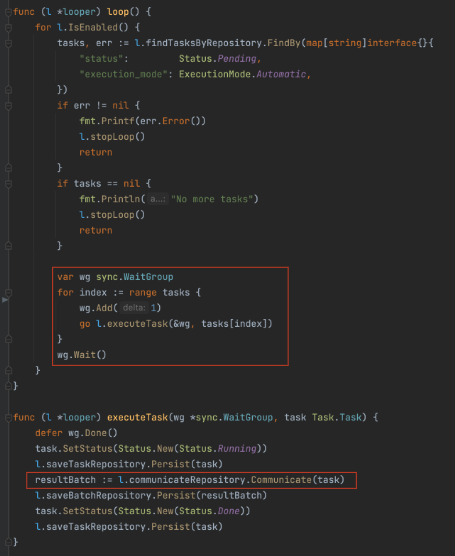
\includegraphics[height=0.3\textheight]{./part/Ejecucion/Seguimiento/Testing/img/Looper}
    \caption{testing looper.go detail}\label{fig:testingLooper}
\end{figure}

el punto clave de la figura \ref{fig:testingLooper} señalado en el recuadro rojo es el adaptador de comunicación GRPC es un adaptador experimental que debido a la inexperiencia en su uso está desarrollado de forma ineficiente. Hemos extraido toda la lógica posible a este servicio que es la parte core:

El adaptador puede tener múltiples errores inesperados, no conseguir comunicar con el servicio cliente, timeouts, malas implementaciones de la librería, pero se ha protegido al dominio de todo esto mediante una interfaz que garantiza que ante cualquier error se devuelve siempre un resultado. Lo único que quedaría por implementar y testear sería que el proceso no consiguiera terminar y se quedara la gorutine en un proceso infinito. para ello en el proceso de descubrimiento del lenguaje sabemos que hay un punto débil en el dominio. No hemos hehco uso de una herramienta de Golang que se conoce como context. que permite gestionar los timeouts de las gorutines evitando que que queden procesos hijos sin control.

Tengamos en cuenta que hemos extraido de toda la comunicación con el cliente una interfaz útil y única para comunicarnos, una lógica de negocio que entender en pocas lineas de código y explicar su funcionamiento, controlarlo y testearlo y aún así encontramos puntos débiles que mejorar en ese diseño. Si a esto le hubieramos sumado las lineas de codigo que hay detrás de la interfaz de comunicacion sería ingestionable. para cuantificar esto vamos a hacer una aproximación al diseño del test necesario para cubrir el adaptador de comunicacion

El código completo se encuentra en el repositorio github. Simplificando para esta explicación el pseudocódigo sería el siguiente

\begin{verbatim}
connection, err := grpc.Dial()
    serverStream:
        client.CallServerStream(request)
        responseStream.Recv()
    Bidirectional:
        client.CallBidirectional()
        async stream.Recv()
        async stream.Send()
        stream.CloseSend()
    ClientStream:
        client.CallClientStream()
        stream.Send
        stream.CloseAndRecv()
    Unary
        client.CallUnary()
connection.Close()
\end{verbatim}

vemos que hay mucha lógica junta, múltiples responsabilidades y por lo tanto no es un buen diseño. Como se demuestra mejor es intentando diseñar los tests. Para empezar extraer del código estas clases de equivalencia y factores no ha sido sencillo ya que hay multiples gestiones de errores dispersos por el código y es un código extenso 178 lineas. Esto ocurre en multitud de ocasiones, ya sea debido al tiempo, desconocimiento o mala praxis nos encontramos con códigos de esta magnitud. La arquitectura y todo este proceso lo que hace es protegernos de estas secciones sucias.

factores y posibles respuestas:

\begin{itemize}
    \item grpc.Dial(): err, connection
    \item client.CallServerStream(request): err,stream
    \item responseStream.Recv(): EOF,err,nil
    \item client.CallBidirectional(): error,stream
    \item stream.Recv(): EOF,err, result
    \item stream.Send(): EOF, nil,err
    \item stream.CloseSend() err,nil
    \item client.CallClientStream(): err, stream
    \item stream.Send: err, nil
    \item stream.CloseAndRecv(): err, nil
    \item client.CallUnary(): err,nil
    \item connection.Close(): err, nil
\end{itemize}

Si no entendieramos bien el concepto de clase de equivalencia podría llevarnos a un mal diseño de los tests o a hacerlo más complejo. Aunque hay factores que tiene tres respuestas posibles EOF y nil tienen que ir de la mano, significa que no ha habido error, primero obtienes un nil en el error y luego obtienes un error tipo EOF que significa que todo ha terminado correctamente. y luego tenemos cuando obtenmos un error distinto de EOF, si esto ocurre nos importa cuaántas veces haya ocurrido el caso sin error, será error igualmente. Con lo cual las clases de equivalencia serían

\begin{itemize}
    \item grpc.Dial(): err, connection
    \item client.CallServerStream(): err,stream
    \item responseStream.Recv(): nil\&EOF,err
    \item client.CallBidirectional(): error,stream
    \item stream.Recv(): nil\&EOF,err
    \item stream.Send(): nil\&EOF,err
    \item stream.CloseSend() err,nil
    \item client.CallClientStream(): err, stream
    \item stream.Send: err, nil
    \item stream.CloseAndRecv(): err, nil
    \item client.CallUnary(): err,nil
    \item connection.Close(): err, nil
\end{itemize}

para este caso tendríamos \[ 2^{12} = 4096 \] combinaciones posibles que pairwise reduce a 59 tests. aquí se ve la potencia del método. Volviendo posible un testing con ciertas garantías incluso en un código como el que nos ocupa.
